\title{%
  Inmatning och felhantering
}
\author{Daniel Bosk}
\institute{%
  KTH EECS
}

\mode<article>{\maketitle}
\mode<presentation>{%
  \begin{frame}
    \maketitle
  \end{frame}
}

\mode*

\begin{abstract}
  % What's the problem?
% Why is it a problem? Research gap left by other approaches?
% Why is it important? Why care?
% What's the approach? How to solve the problem?
% What's the findings? How was it evaluated, what are the results, limitations, 
% what remains to be done?

% XXX Summary
\emph{Summary:}
\dots

% XXX Motivation and intended learning outcomes
\emph{Intended learning outcomes:}
\dots

% XXX Prerequisites
\emph{Prerequisites:}
\dots

% XXX Reading material
\emph{Reading:}
\dots

\end{abstract}


\section{Inmatning}

\subsection{Inmatning av text}

\begin{frame}
  \begin{center}
    \mintinline[fontsize=\Large]{python}|variable = input("Optional prompt:")|
  \end{center}
\end{frame}

\begin{frame}[fragile]
  \begin{example}
    \begin{minted}{python}
age = input("How old are you? ")
print(f"Aha, so you're {age} years.")
    \end{minted}
  \end{example}

  \pause

  \begin{example}
    \begin{minted}{python}
print("How old are you?", end=" ")
age = input()
print(f"Ah, you're only {age} years old.")
    \end{minted}
  \end{example}
\end{frame}

\subsection{Inmatning av andra typer}

\begin{frame}
  \begin{remark}[\mintinline{python}|input()|]
    \begin{itemize}
      \item Returnerar en sträng.
      \item Måste typkonvertera om man vill ha annat.
    \end{itemize}
  \end{remark}
\end{frame}

\begin{frame}[fragile]
  \begin{example}[Funkar inte]
    \begin{minted}{python}
age = input("How old are you?")
print(f"Ah, then I'm older, I'm {age+1}!")
    \end{minted}
  \end{example}

  \pause

  \begin{example}[Funkar]
    \begin{minted}[highlightlines=2]{python}
age = input("How old are you?")
print(f"Oh, then I'm older, I'm {int(age)+1}!")
    \end{minted}
  \end{example}

  \begin{example}[Funkar]
    \begin{minted}[highlightlines=1]{python}
age = int(input("How old are you?"))
print(f"Oh, then I'm older, I'm {age+1}!")
    \end{minted}
  \end{example}
\end{frame}

\section{Datatyper och operationer}

\begin{frame}
  \begin{remark}[Inbyggda datatyper]
    \begin{itemize}
      \item \mintinline{python}|str(x)| gör om \mintinline{python}|x| till textsträng
      \item \mintinline{python}|int(x)| gör om till heltal
      \item \mintinline{python}|float(x)| gör om till flyttal
      \item \mintinline{python}|complex(re, im)| gör om till komplext tal
    \end{itemize}
  \end{remark}
\end{frame}


\subsection{Numeriska typer}

\begin{frame}[fragile]
  \begin{block}{Operationer numeriska typer}
    \begin{itemize}
      \item \mintinline{python}|a + b| ger addition
      \item \mintinline{python}|a - b| ger subtraktion
      \item \mintinline{python}|a * b| ger multiplikation
      \item \mintinline{python}|a / b| ger division (heltal till flyttal)
      \item \mintinline{python}|a // b| ger heltalsdivision (heltal till heltal)
      \item \mintinline{python}|a % b| ger resten vid heltalsdivision
      \item \mintinline{python}|a ** b| ger \(a^b\)
    \end{itemize}
  \end{block}
\end{frame}


\section{Fel och felhantering}

\subsection{Särfall}

\begin{frame}[fragile]
  \begin{example}
    \begin{minted}{text}
>>> int("a")
Traceback (most recent call last):
  File "<stdin>", line 1, in <module>
ValueError: invalid literal for int() with base 10: 'a'
>>> 
    \end{minted}
  \end{example}
\end{frame}

\begin{frame}[fragile]
  \begin{example}
    \begin{minted}{text}
>>> 5/0
Traceback (most recent call last):
  File "<stdin>", line 1, in <module>
ZeroDivisionError: division by zero
>>> 
    \end{minted}
  \end{example}
\end{frame}

\begin{frame}[fragile]
  \begin{example}
    \begin{minted}{text}
>>> prynt(3)
Traceback (most recent call last):
  File "<stdin>", line 1, in <module>
NameError: name 'prynt' is not defined
>>> 
    \end{minted}
  \end{example}
\end{frame}

\subsection{Felhantering: att fånga särfall}

\begin{frame}
  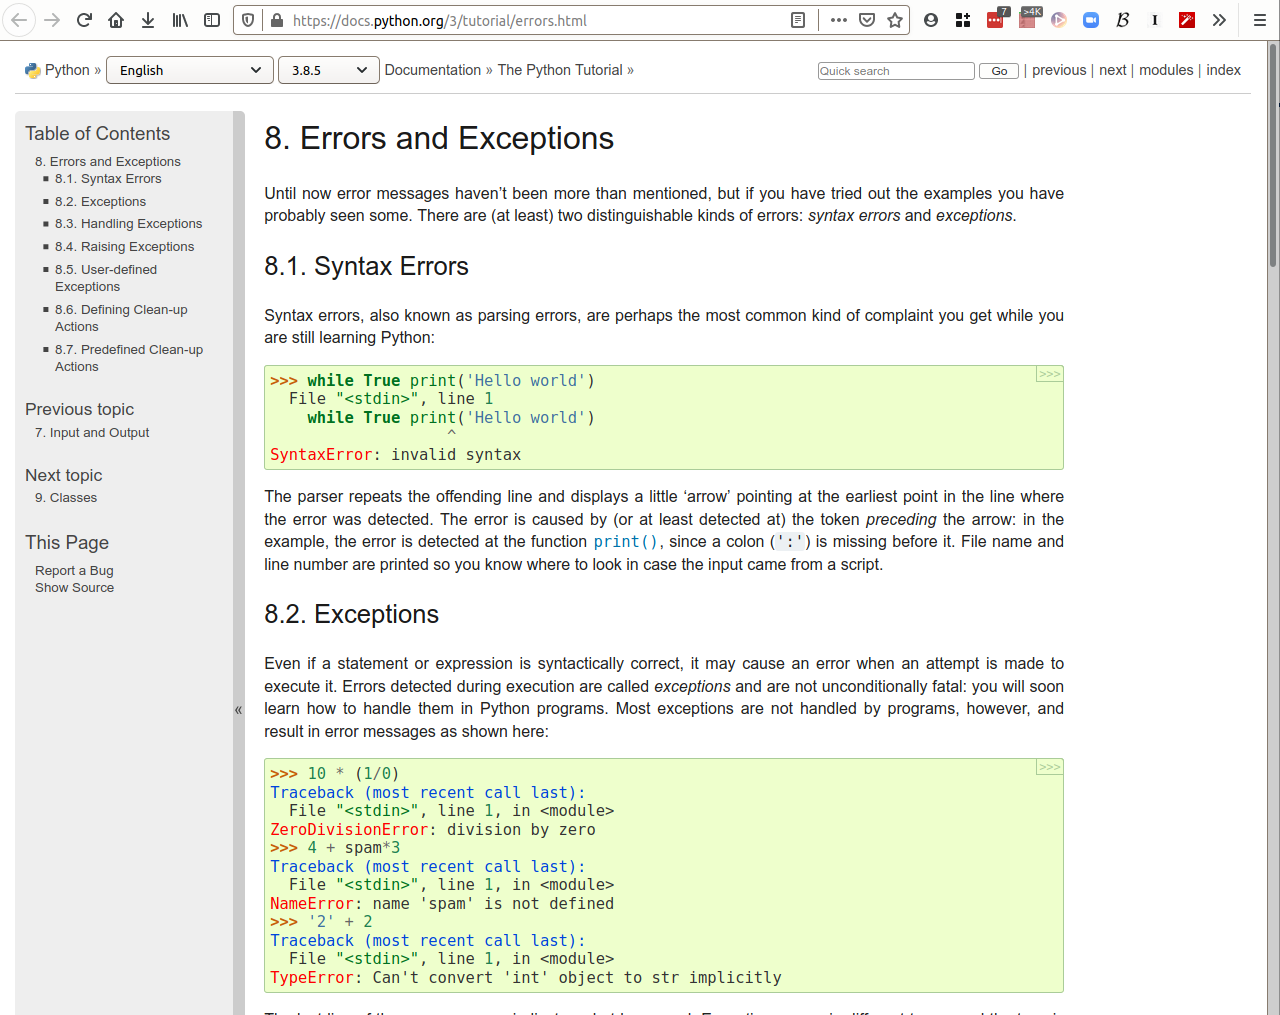
\includegraphics[width=\columnwidth]{figs/docs-except.png}
\end{frame}

\begin{frame}[fragile]
  \begin{example}[Fånga särfall: valuerr.py]
    \inputminted{python}{examples/valuerr.py}
  \end{example}

  \pause

  \begin{example}
    \begin{minted}{text}
$ python3 valuerr.py
We caught this: invalid literal for int() with base 10: 'a'
    \end{minted}
  \end{example}
\end{frame}

\begin{frame}[fragile]
  \begin{minted}{python}
try:
  # kod som kan orsaka fel
except Exception as err:
  print(f"Ett okänt fel inträffade: {err}")
  \end{minted}
  \begin{remark}
    \begin{itemize}
      \item \mintinline{python}{except Exception as err} fångar \emph{allt}!
    \end{itemize}
  \end{remark}
\end{frame}

\begin{frame}[fragile]
  \begin{example}[manyerr.py]
    \inputminted{python}{examples/manyerr.py}
  \end{example}
\end{frame}

